\documentclass[oneside,a4paper]{mecom}
% Preamble
\usepackage{graphicx}
\usepackage[spanish]{babel}
\usepackage{amsmath,amsfonts}
\usepackage{url}
\usepackage{overcite}
\usepackage{times}
\usepackage{bm}
\usepackage{multicol}
\usepackage{colortbl}

\pagestyle{empty}
\setlength{\textwidth}{16cm}
\setlength{\textheight}{21cm}
\setlength{\oddsidemargin}{-0.04cm}
\setlength{\topmargin}{18.1mm}
\setlength{\headheight}{0mm}
\setlength{\headsep}{0mm}


\title{COMPUTACI\'ON DE ALTO RENDIMIENTO EN EL ESTUDIO DE REACCIONES QU\'IMICAS EN SOLUCIONES A TRAV\'ES DE M\'ETODOS CL\'ASICOS Y CU\'ANTICOS}
\author{
\textbf{P. Listingart\stared, E. Mocskos\stared, M.C. Gonz\'alez Lebrero\dagged and D. Estrin\dagged}\\
\\
\stared Laboratorio de Sistemas Complejos\\
Departamento de Computaci\'on, Facultad de Ciencias Exactas y Naturales (FCEyN)\\
Universidad de Buenos Aires, Ciudad Universitaria, \\
Pabell\'on I, (C1428EGA) Buenos Aires, Argentina.\\
web page: http://www.lsc.dc.uba.ar\\
\dagged Departamento de Qu\'imica Inorg\'anica, Anal\'itica y Qu\'imica F\'isica, \\
Facultad de Ciencias Exactas y Naturales (FCEyN), \\
Universidad de Buenos Aires, Ciudad Universitaria, \\
Pabell\'on I, 1428 Buenos Aires, Argentina.
}

\begin{document}
\vspace{3cm}
\maketitle
\noindent\textbf{Key Words:} HPC, Cluster, Perfomance, C\'alculo Paralelo, Beowulf, M\'etodos h\'ibridos.
\vspace{12pt}

\begin{abstract}
En este trabajo se presenta un software de c\'omputo de alto rendimiento aplicado a la simulaci\'on de reactividad qu\'imica en soluci\'on. El m\'etodo utilizado para realizar la simulaci\'on se encuadra dentro de un esquema h\'ibrido cu\'antico-cl\'asico (QM-MM) en el cual el solvente es tratado cl\'asicamente (como masas y cargas puntuales) mientras que el soluto es tratado con rigurosidad cu\'antica (DFT, en nuestro caso), de esta manera se logra optimizar el costo computacional ya que se computa la estructura electr\'onica s\'olo de la porci\'on del sistema en la que es realmente relevante. El proyecto consiste en la construcci\'on de un software paralelo de simulaci\'on num\'erica a partir de una versi\'on serial preexistente y su implementaci\'on en un cluster Beowulf, en el estudio y predicci\'on de reacciones qu\'imicas en soluci\'on. La combinaci\'on del hardware y software mencionado y el an\'alisis de distintas estrategias de paralelizaci\'on (incluyendo diversas modalidades de pasaje de mensajes) permitir\'an la resoluci\'on de problemas m\'as realistas y previamente inabordables, obteniendo un algoritmo escalable.
\end{abstract}

\newpage

\section{Introducci\'on}
La simulaci\'on en qu\'imica es una herramienta cada vez m\'as utilizada. 
El desarrollo de t\'ecnicas refinadas, as\'i como el aumento geom\'etrico del poder de c\'omputo son dos de las razones m\'as importantes de su creciente uso.
Ya sea como complemento o como reemplazo de experimentos, la simulaci\'on aporta, entre otras cosas, una visi\'on microsc\'opica inalcanzable por otra v\'ia.

Las metodolog\'ias utilizadas en simulaci\'on var\'ian seg\'un el problema a tratar. En general, se dividen en dos grandes ramas, la llamada rama \emph{cl\'asica} y la llamada \emph{cu\'antica}. 
La mec\'anica que rige el comportamiento de part\'iculas peque\~nas (c\'omo los electrones) es la llamada mec\'anica cu\'antica, que fue desarrollada a principios del siglo pasado por f\'isicos ilustres como Einstein, Planck, Bhory otros. 
Lamentablemente no existe una forma exacta de resolver las ecuaciones asociadas a esta mec\'anica, y las soluciones aproximadas accesibles son muy demandantes desde el punto de vista computacional.
Esta elevada demanda hace prohibitivo el uso de esta t\'ecnica a sistemas con un n\'umero elevado de \'atomos.

Por otro lado la mec\'anica cl\'asica, menos demandante, es incapaz de representar electrones, por lo que solo puede utilizarse si la distribuci\'on de los mismos no cambia.
No es posible, entonces, tratar reacciones qu\'imicas (donde la distribuci\'on electr\'onica cambia considerablemente).

Si se quieren tratar reacciones en soluci\'on, se encuentra el problema de que el n\'umero de \'atomos es demasiado grande como para tratarlo con rigurosidad cu\'antica, sin embargo, al haber reacci\'on qu\'imica, no se puede utilizar una metodolog\'ia totalmente cl\'asica.
Por ello se han desarrollado las metodolog\'ias h\'ibridas\cite{Diaz2001,Nemukhin2002,Kesavan2003}, donde a una peque\~na porci\'on del sistema (la parte reactiva), se la trata con la metodolog\'ia cu\'antica, mientras que al resto se lo trata como un campo de fuerzas cl\'asico.

\section{Metodolog\'ia}

El desarrollo de un programa paralelo tiene como objetivo no s\'olo optimizar una \'unica m\'etrica, como puede ser el tiempo de ejecuci\'on total.
Un buen dise\~no debe, adem\'as, optimizar una funci\'on dependiente del problema a resolver donde se tienen en cuenta el tiempo de ejecuci\'on, los requerimientos de memoria, los costos de implementaci\'on y mantenimiento de la soluci\'on, entre otros. 
Estas optimizaciones en el dise\~no conllevan una tensi\'on entre simplicidad, performance, portabilidad y otros factores.

Partiendo de un programa serial pre existente \cite{lebrero2002} y para poder decidir c\'omo encarar estas optimizaciones, se debi\'o realizar un estudio de la complejidad y del comportamiento del programa serial. 
Para ello realizamos un profiling utilizando diversas herramientas provistas por el sistema operativo Linux y por el compilador $g77$ utilizado.

El esquema de aproximaci\'on implementado en la versi\'on serial est\'a basado en la teor\'ia del funcional de la densidad (DFT), en la cual la variable fundamental es la densidad electr\'onica. 
Esta variable, $r$, se expande con un conjunto de funciones base.

\begin{displaymath}
\rho = \sum_{i=1}^N \mid X_i^{KS} \mid^{2}
\end{displaymath}

Se puede escribir la energ\'ia total como:

\begin{displaymath}
E[\rho] = -\frac{1}{2}\langle X_i^{KS}\mid \sum_i\sigma_i^{2} \mid X_i^{KS}\rangle + \int v(r) \rho(r) dr + \frac{1}{2}\int \int \frac{\rho(r_{1})\rho(r_{2})}{r_{12}}dr_{1}dr_{2}+E_{xc}[\rho]
\end{displaymath}

La parte m\'as costosa del c\'alculo esta relacionada con los dos \'ultimos t\'erminos de esta expresi\'on, son ellos los correspondientes a la energ\'ia de repulsi\'on de Coulomb, y el t\'ermino de intercambio y correlaci\'on.

El primer termino es calculado en forma anal\'itica, pero su costo del orden de $N^3$, donde $N$ est\'a directamente relacionada con el tama\~no del sistema.
Este t\'ermino consiste de $N^3$ integrales anal\'iticas que se pueden calcular en forma independiente, por lo que se puede paralelizar con facilidad.

El segundo t\'ermino se debe evaluar en forma num\'erica, empleando un esquema de integraci\'on en una grilla centrada en los \'atomos y tambi\'en escala como $N^3$. 
Este t\'ermino es paralelizable entre los distintos procesos separando el dominio sobre el que se calcula la integral.

En el profiling realizado veremos que el c\'omputo de estos dos t\'erminos representa m\'as del 90\% del costo computacional total, ya que el costo de los dos primeros t\'erminos escala con $N^2$.

\subsection{Profiling}
A continuaci\'on observaremos los datos obtenidos de la realizaci\'on del profiling del programa serial.
En la figura \ref{fig:Profiling} se detallan los porcentajes de procesamiento que insume cada subrutina en una corrida.

\begin{figure}[ht!]
\begin{center}
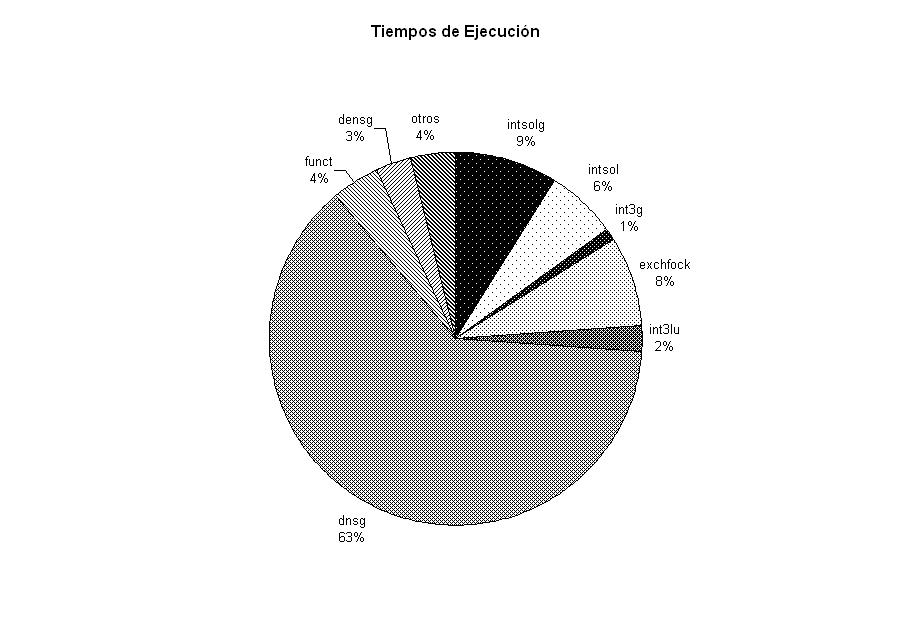
\includegraphics[keepaspectratio, width=14cm]{Profiling2}
\end{center}
\caption[Porcentajes de tiempo consumidos por las rutinas]{\small{Porcentajes de tiempo consumidos por las rutinas.}}
\label{fig:Profiling}
\end{figure}

Con estos resultados pudimos identificar cu\'ales eran las rutinas que conven\'ia analizar para evaluar su posible paralelizaci\'on.

Se puede observar en la figura \ref{fig:Profiling} que si bien la rutina \textsf{dnsg} insume un 62.5\% del tiempo de procesamiento total, esto se debe a la cantidad de veces que es invocada, ya que en cada invocaci\'on su tiempo de procesamieto es casi cero, es decir despreciable respecto de otras. 
Lo mismo ocurre con las rutinas \textsf{exchfock}, {\textsf{funct} y \textsf{densg}.

Siguiendo con los resultados del profiling realizado, se buscaron las llamadas correspondientes a las rutinas que calculan la densidad electr\'onica ya que las mismas en las corridas son las que insumen mayor cantidad de tiempo de procesamiento. 
Al realizar esta b\'usqueda se encontraron las rutinas \textsf{exchfock}, \textsf{exhnum}, \textsf{exhnumop}, \textsf{exchnum2} y \textsf{exchnum2op}.

Es en estas cinco \'ultimas rutinas es en las que se centra nuestro an\'alisis de paralelizaci\'on. 
Se podr\'a observar m\'as adelante que las cinco efect\'uan el mismo tipo de c\'alculo, variando s\'olo en algunos detalles internos como ser utilizaci\'on o no de una matriz resultado, o la cantidad de par\'ametros de salida que tienen.

\subsection{Implementaci\'on}

En primera instancia se reorganiz\'o el c\'odigo de manera de eliminar vicios de programaci\'on y lograr evitar ciertos problemas que pueden traer aparejadas algunas reglas de utilizaci\'on del fortran. 
Por ejemplo, al utilizar declaraci\'on impl\'icita de variables si el programador declara que las variables que empiecen con letras de la \texttt{A} a la \texttt{H} ser�n del tipo \texttt{REAL*8} pero luego ante un descuido declara otra variable \texttt{INTEGER} con alg\'un nombre que empiece entre esas letras podr\'an darse errores o diferencias en los resultados. 
En etapas posteriores se fueron eliminando las declaraciones impl\'icitas de variables y se constat\'o mediante un $dump$ del estado del programa que no se hubiera modificado nada respecto a la versi\'on serial.

La paralelizaci\'on del algoritmo se realiza a trav\'es de la descomposici\'on del dominio de la integral. 

Cada uno de los procesos participantes, tiene en memoria el dominio completo y realiza sobre el subdominio correpondiente sus c\'alculos en forma local.
Finalmente, como es necesario para las operaciones subsiguientes contar con el total de los datos, se realiza la sincronizaci\'on con todos los procesos.

Como se mencion\'o con anterioridad al realizar el profiling se observ\'o que entre un 65\% y 75\% del tiempo era consumido por las rutinas de tipo \textsf{densg} que son las encargadas de calcular los gradientes necesarios para obtener el valor en cada punto de la grilla de trabajo.

Esta rutinas en s\'i consumen muy poco tiempo de ejecuci\'on, pero el problema es que son llamadas en el orden de los millones de veces.

Por lo tanto, se buscaron las rutinas desde donde \textsf{dnsg}(y las otras rutinas similares) eran llamadas.
Esto ocurre en las funciones de tipo \textsf{exch}(\textsf{exchfock}, \textsf{exchnum}, \textsf{exchnum2}, \textsf{exchnum2op}).
En las mismas se observ\'o que las llamadas se encontraban dentro de tres ciclos, con los cuales se armaban los puntos de la grilla para cada \'atomo del sistema.
Se decidi\'o paralelizar por el ciclo m\'as externo, que justamente es el que itera por cada \'atomo, para evitar sobrecarga de comunicaci\'on entre los nodos.

En este caso, si el n\'umero de procesos utilizados es menor que el n\'umero de \'atomos con los que se trabaja se dividen los mismos de manera uniforme. 
En cambio, si hay m\'as procesos que \'atomos, todo el procesamiento va a un solo nodo, lo cual produce p\'erdidas con respecto al modelo original por la sobrecarga de comunicaci\'on e inicializaci\'on del sistema paralelo.

En cuanto a las modificaciones realizadas al sistema, en el archivo \textsf{main.f} se agregaron sentencias de MPI \cite{Pacheco96, mpich-install},  para la inicializaci\'on y finalizaci\'on de la utilizaci\'on de la librer\'ia que lo implementa. Se utiliz\'o la librer\'ia \textsf{MPICH}\cite{MPICH} para las pruebas realizadas.

En cada uno de los archivos \textsf{exch} se agregaron instrucciones para calcular el n\'umero de procesadores a utilizar de acuerdo a los \'atomos presentes en el sistema, otras para enviar los resultados obtenidos hacia el proceso 0 (o simplemente \emph{root}) en caso de no serlo y para recibir de todos los procesos los resultados (en caso de ser el \emph{root}).

Las llamadas a rutinas de salida debieron ser eliminadas para los procesos distintos al \emph{root} para que el mismo fuera el \'unico en realizar la escritura de datos de salida.

\section{Resultados y Discusi\'on}

\textbf{el de 7 �tomos es un peroxinitrito (OONO) mas un di�xido de carbono (CO2) cuanticos mas 498 mol�culas de agua}

\textbf{el de 4 �tomos es s�lo el peroxinitrito con las 498 mol�culas de agua}

Las corridas en todos los casos fueron realizadas con iguales par\'ametros de entrada variando solamente la cantidad de pasos entre las mismas. El sistema const\'o de siete \'atomos yfue armado de forma tal de que se pudiera tener una distribuci\'on casi uniforme de los dominios sobre los procesos.

\begin{table}
\begin{center}
\begin{tabular}{|c|c|c|c|c|c|}
\hline
\ & \textbf{1000 pasos} & \textbf{3000 pasos}& \textbf{5000 pasos}& \textbf{7000 pasos}& \textbf{10000 pasos}\\
\hline
\texttt{Serial} & 01:40	& 05:10	& 09:10	& 12:30 & 19:54	\\
\texttt{Paralelo}  & 01:38 & 04:50 & 08:12 & 11:29 & 16:30\\
\hline
\end{tabular}
\end{center}
\caption[Tiempos de ejecuci\'on en m\'aquina SMP]{\small{Tiempos de ejecuci\'on total del programa en una m\'aquina SMP Xeon Dual. Los resultados est\'an expresados en minutos.}}
\label{tab:TiemposEjecucion1}
\end{table}

Una vez realizadas las modificaciones se realizaron corridas en una m\'aquina SMP XEON Dual, obteni\'endose los resultados de la tabla \ref{tab:TiemposEjecucion1}.
La misma puede observarse de mejor manera en la figura \ref{fig:Papita}

\begin{figure}[ht!]
\begin{center}
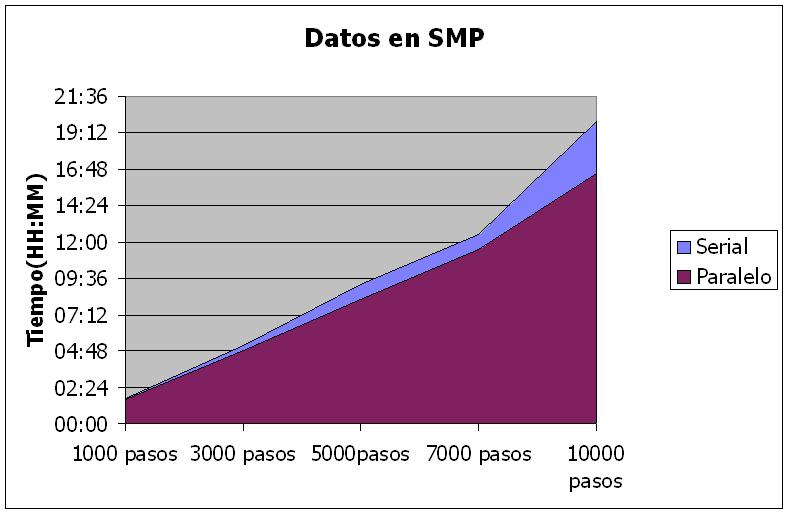
\includegraphics[keepaspectratio, width=14cm]{Papita}
\end{center}
\caption[Tiempos de ejecuci\'on en m\'aquina SMP]{\small{Tiempos de ejecuci\'on total del programa en una m\'aquina SMP Xeon Dual. Los resultados est\'an expresados en minutos.}}
\label{fig:Papita}
\end{figure}


Luego se realizaron mediciones en el cluster $Rocky$ del Laboratorio de Sistemas Complejos de la Facultad de Ciencias Exactas y Naturales de la UBA. El mismo est\'a compuesto por cuatro nodos AMD Opteron duales conectados por una red de Gigabit Ehernet. 
Las corridas fueron realizadas con cuatro procesos en nodos distintos, es decir a raz\'on de un proceso en cada nodo, obteni\'endose los resultados que se pueden ver en la tabla \ref{tab:TiemposEjecucion2}.

\begin{table}
\begin{center}
\begin{tabular}{|c|c|c|c|}
\hline
\ & \textbf{1000 pasos} & \textbf{3000 pasos}& \textbf{5000 pasos}\\
\hline
\texttt{Serial} & 01:59	& 05:56	& 09:46	\\
\texttt{Paralelo}  & 01:56 & 05:49 & 09:26 \\
\hline
\end{tabular}
\end{center}
\caption[Tiempos de ejecuci\'on total del programa en 4 procesos]{\small{Tiempos de ejecuci\'on total del programa en 4 procesos.}}
\label{tab:TiemposEjecucion2}
\end{table}

\begin{figure}[ht!]
\begin{center}
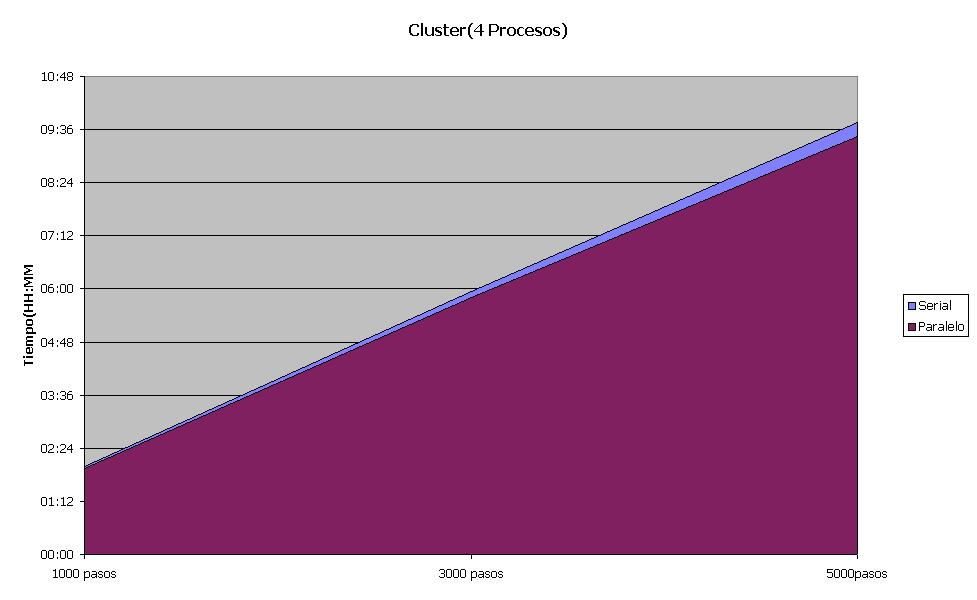
\includegraphics[keepaspectratio, width=14cm]{Rocky1}
\end{center}
\caption[Tiempos de ejecuci\'on total del programa en 4 procesos]{\small{Tiempos de ejecuci\'on total del programa en 4 procesos.}}
\label{fig:Rocky1}
\end{figure}



Finalmente fueron realizadas las mismas ejecuciones sobre el mismo cluster pero utilizando uncamente dos procesos en nodos distintos, obteniendose los siguientes resultados visibles en la tabla \ref{tab:TiemposEjecucion3}.

\begin{table}
\begin{center}
\begin{tabular}{|c|c|c|c|}
\hline
\ & \textbf{1000 pasos} & \textbf{3000 pasos}& \textbf{5000 pasos}\\
\hline
\texttt{Serial} & 01:59	& 05:56	& 09:46	\\
\texttt{Paralelo}  & 01:57 & 05:53 & 09:36 \\
\hline
\end{tabular}
\end{center}
\caption[Tiempos de ejecuci\'on total del programa en 2 procesos]{\small{Tiempos de ejecuci\'on total del programa en 2 procesos.}}
\label{tab:TiemposEjecucion3}
\end{table}

\begin{figure}[ht!]
\begin{center}
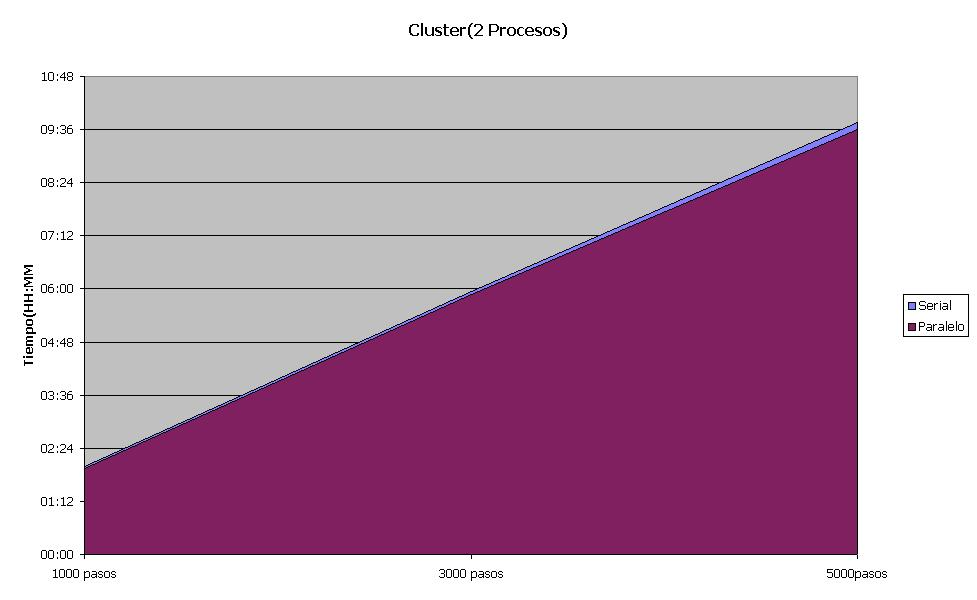
\includegraphics[keepaspectratio, width=14cm]{Rocky2}
\end{center}
\caption[Tiempos de ejecuci\'on total del programa en 2 procesos]{\small{Tiempos de ejecuci\'on total del programa en 2 procesos.}}
\label{fig:Rocky2}
\end{figure}

Una vez obtenidos los datos de las ejecuciones del sistema en distintas configuraciones y entornos se pudieron obtener datos sobre $Speedup$, $Overhead$ y $Eficiencia$, observables en las figuras \ref{fig:Speedup}, \ref{fig:Overhead} y \ref{fig:Eficiencia}

\begin{figure}[ht!]
\begin{center}
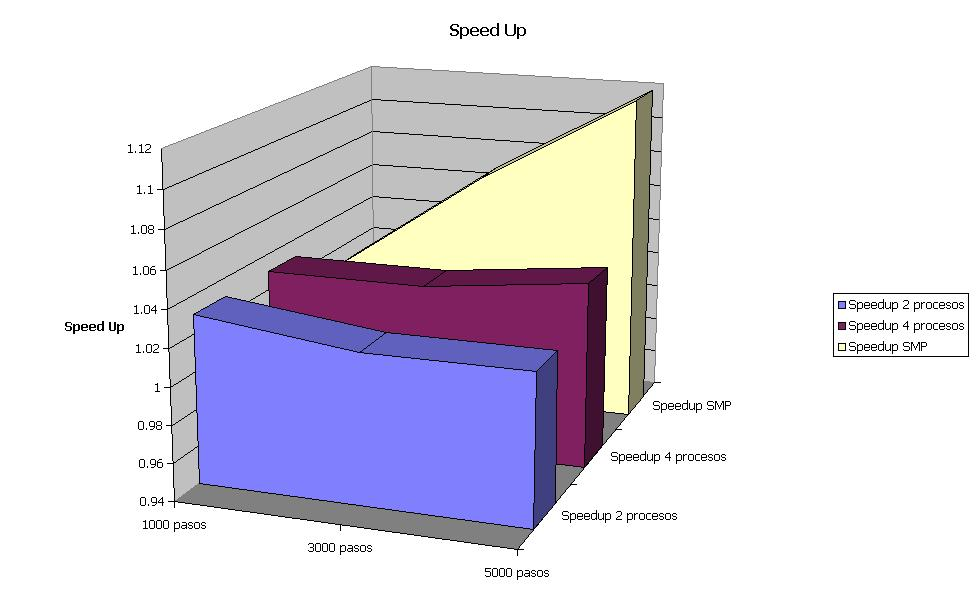
\includegraphics[keepaspectratio, width=14cm]{Speedup}
\end{center}
\caption[Comparaci\'on del Speedup obtenido en las distintas configuraciones]{\small{Comparaci\'on del Speedup obtenido en las distintas configuraciones.}}
\label{fig:Speedup}
\end{figure}

\begin{figure}[ht!]
\begin{center}
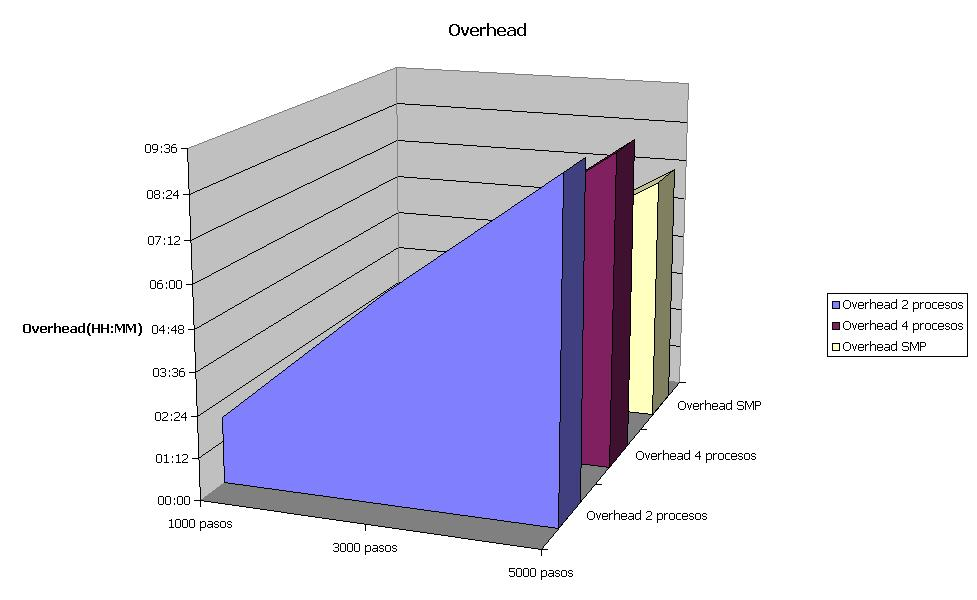
\includegraphics[keepaspectratio, width=14cm]{Overhead}
\end{center}
\caption[Comparaci\'on del Overhead obtenido en las distintas configuraciones]{\small{Comparaci\'on del Overhead obtenido en las distintas configuraciones.}}
\label{fig:Overhead}
\end{figure}

\begin{figure}[ht!]
\begin{center}
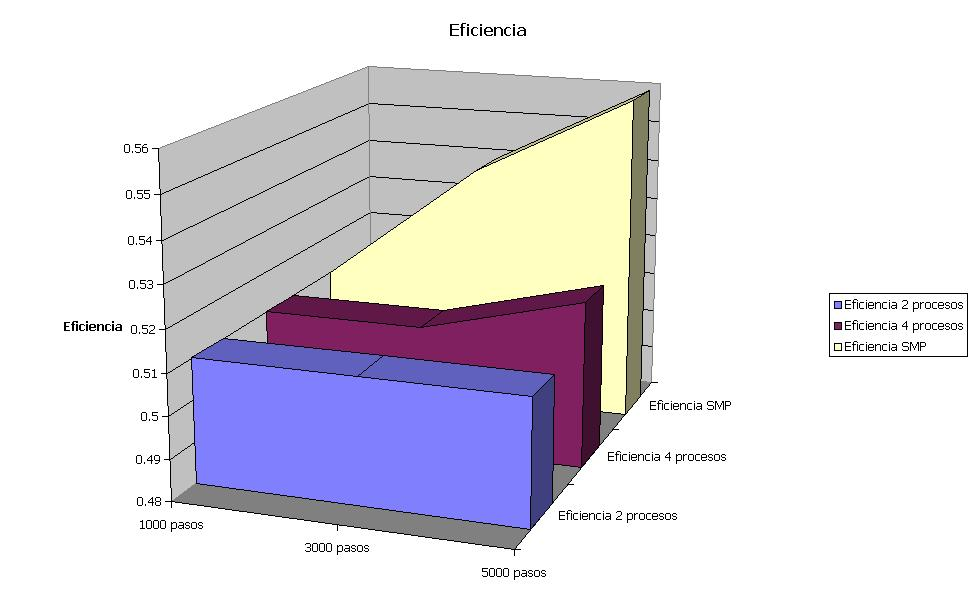
\includegraphics[keepaspectratio, width=14cm]{Eficiencia}
\end{center}
\caption[Comparaci\'on de la eficiencia obtenida en las distintas configuraciones]{\small{Comparaci\'on de la eficiencia obtenida en las distintas configuraciones.}}
\label{fig:Eficiencia}
\end{figure}


Puede observarse que conforme el dominio del problema crece la brecha entre los tiempos del sistema serial y los del paralelo se vuelven mayores. Quedar\'a a futuro la ejecuci\'on de un sistema de mayores dimensiones para completar el estudio sobre performance del sistema paralelizado. A simple vista puede observarse que para mayores dominios del problema la performance del sistema paralelo crece con respecto al serial. 

En contraparte a los resultados obtenidos puede observarse el gran overhead introducido en la versi\'on paralela del programa debido al pasaje de mensajes, lo cual hace que el $Speedup$ no sea lineal con respecto a la cantidad de procesos utilizados. Esto quiere decir que si el $Speedup$ fuera lineal, utilizando dos procesos el c\'alculo deber\'ia tardar la mitad de tiempo. \'esta situaci\'on no se esta cumpliendo debido a que el overhead es pr\'acticamente la mitad del total del tiempo, y a futuro queda una investigaci\'on m\'as profunda para intentar reducir el overhead.

Como trabajo a futuro se testear\'an dominios mayores y la ejecuci\'on de los mismos en un cluster de mayor magnitud, sin embargo esto no puede ser realizado de momento debido a falta de tiempo para realizar ejecuciones de gran envergadura. 

Por otra parte podr\'ia investigarse a futuro la utilizaci\'on de mensajes no bloqueantes, ya que la metodolog\'ia actual (paso de mensajes bloqueantes) produce un overhead en el cual los procesos se encuentran inactivos. Sin embargo, la implementaci\'on de mensajes no bloqueantes requiere de un an\'alisis exhaustivo del problema para poder seleccionar zonas del programa en el que puedan solaparse c\'alculo y comunicaci\'on. Dado que la funci\'on que ha sido elegida como blanco de optimizaci\'on no requiere sincronizaci\'on intermedia, por el momento no hemos utilizado esta modalidad.

\section{Conclusiones}

Como pudo observarse, el algoritmo paralelo se vuelve m\'as efectivo conforme el dominio del problema crece. Esto se debe a que el overhead producido por la comunicaci\'on entre procesos se ve compensado por la cantidad de instrucciones ejecutadas en cada uno de los nodos. 


El programa paralelo obtenido abre un abanico de posibilidades para poder resolver sistemas intratables hasta el momento, he aqu\'i su mejor caracter\'istica. 
Adicionalmente, la performance del programa resulta razonable y el overhead producido se ve compensado por la ventaja de poder tratar sistemas cada vez m\'as grandes.

\bibliographystyle{mecom}
\bibliography{complex_2005_09_12}

\end{document}